\documentclass[12pt]{article}

\usepackage[utf8]{inputenc}
\usepackage[english]{babel}
\usepackage{sectsty}
\usepackage{multicol, caption}
\usepackage{graphicx}
\usepackage{wrapfig}
\usepackage{subfig}
\usepackage{subcaption}
%\usepackage{biblatex}
\usepackage[margin=0.5in]{geometry} % don't know what size margins to use
\BeforeBeginEnvironment{minipage}{\par\vspace{5mm}}
\newenvironment{Figure}
  {\par\medskip\noindent\minipage{\linewidth}}
  {\endminipage\par\medskip}

\setlength{\columnsep}{1cm}
%\addbibresource{paper.bib}
%\nocite{*}
\sectionfont{\fontsize{12}{15}\selectfont}
 

\begin{document}
    \begin{center}
        \textbf{Evaluation of Classifiers and Feature Selection on Spam Filtering test} 
    \end{center}

    \begin{center}
        Griffin Dunn and William Thompson
    \end{center}

    \textbf{Abstract:} 
        In this paper we explore the effects of extracting features that are not 
        solely based on word frequency and the selection of classifier for the task
        of determining if a message is spam or not spam (ham). These methods
        will be tested on a publicly available corpora and compared to the results
        of other models introduced by other authors. Classifiers will be selected
        from the variety available through the open-source Python module scikit-learn.

    \begin{multicols}{2}
        \section{Introduction}
            The classification of spam emails is an important task in today's society,
            as we receive potentially hundreds of them a year which clutter
            an already full inbox. These emails also pose a threat to the uninformed
            as many ask for personal information, such as street addresses and banking details.
            Traditionally emails have been filtered through rule-based systems that
            could be reverse engineered to still allow for spam email to get through.
            Some newer filters take advantage of machine learning techniques and use
            them in conjunction with the tradition method which leads to good results,
            but still some emails get through. Some newer classifiers may hold the
            key to filtering out even the most engineered emails to get past a filter.
            
            
            As machine learning has had a resurgence a variety
            of new classifier algorithms and implementations have surfaced that 
            make it quick and easy to implement one of these systems. Along with this
            an explosion of open-source libraries have made difficult parsing tasks
            such as handling raw email data trivial. With this boom, public corpora
            have been created through crowd sourcing, which allow individuals to
            test their ideas on realistic data.

            \begin{Figure}
                \centering
                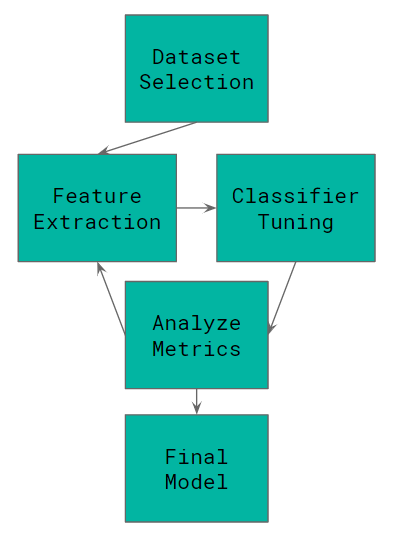
\includegraphics[width=\linewidth]{figures/process.png}
                \captionof{figure}{Our Machine Learning Process}
                \label{fig:process}
            \end{Figure}


            In this paper we explore the selection public datasets, data preparation,
            feature extraction and finally the selection and tuning of classifiers.
            We will do this following the process illustrated in Figure \ref{fig:process}.
        \section{Dataset Selection}
            The correct selection of a dataset was crucial to the testing of 
            different types of features. There were many characteristics that were
            on our `wishlist.' Such as having the freedom of processing 
            the raw text ourselves and determining what features may be important, 
            and not have the data preproccesed or turned into vectors.
            Next we wanted data that was conversational, that didn't use too much 
            slang or leetspeak and was in general proper English. The size of the
            dataset needed to be fairly large, at least 1000, for frequency analysis.
             Lastly, we would like a dataset that was referenced in multiple papers to make comparisons
            of our results to others. So we shortlisted a few datasets that fulfilled
            some of these characteristics.

            The UCI SMS Spam Dataset is a collection of conversational text messages
            origninating from a variety of sources.

            TODO: needed info?

        \section{Data Preparation}
            
            TODO: methodology


            \begin{Figure}
                \centering
                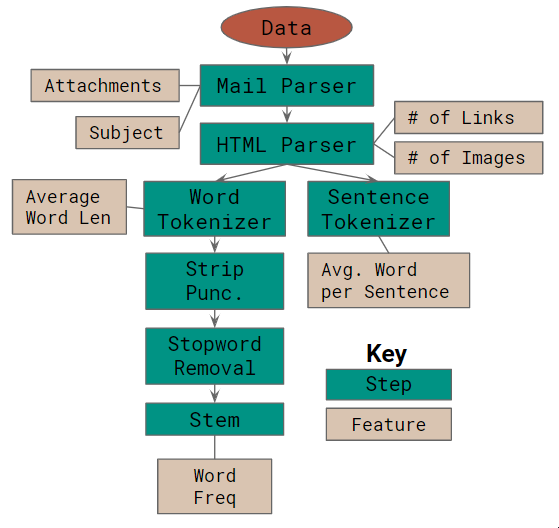
\includegraphics[width=\linewidth]{figures/prep.png}
                \captionof{figure}{Preparation Process}
                \label{fig:preprocess}
            \end{Figure}


            Once data was loaded in we started by running the data the data through
            the Python Standard Library's mail parser, which striped the mail headers
            and put them into a map for separate analysis. It also handled multi-part
            data as files were encoded into the file in base64, and allowed us to count
            the amount of attachments. Without using a mail
            parser it would be difficult to just get the body of the text which
            would be used for feature extraction. Other papers left this data in the
            email, possibly because this information is hard to extract and the tools
            weren't as easily accessible when their implementation was written. We
            decided to strip this data out as to not add noise and also because many 
            headers were left on from other spam checkers, identifying whether or not
            it believed the message was spam or ham.


            Next we used BeautifulSoup's HTML parser to interpret any HTML data that
            was in an email. We queried the document structure for the \textit{href}
            attribute because it indicates a link. Not only an \textit{a} tag can include
            a link, tags such as an \textit{img} tag can also contain one. Potential attackers
            may also use an \textit{a} tag to make a link look like it is going somewhere else,
            such as having the text \textit{http://google.com} a clickable link to
            \textit{http://mygooglephishingsite.com}, but we didn't see this practice 
            occurring in this dataset so we ignored this potential feature. We also looked at the
            amount of linked pictures, as an attacker may try to get credibility with it's prey
            by introducing fancy graphics. Lastly we extracted the raw content from the HTML,
            ignoring any structure that was present for tokenization.


            The tokenization step was done with NLTK's word and sentence tokenizer.
            The sentence tokens were used for some metrics such as average words per
            sentence and could be used in the future for the analysis of sentence
            structure. The word tokens were stripped of punctuation such as '.',
            '?', '(' and ')', which would litter our unigrams. Next we removed stopwords
            from the provided list of English stopwords in NLTK's corpus. Removing
            these words are necessary as they provide no direct meaning when it comes
            to frequency analysis of the documents and would just provide more noise
            in the classifier. Lastly we
            stemmed the words using NLTK's Porter Stemmer with their extensions to
            Martin Porter's algorithm. This allowed use to remove suffixes such as '-s',
            which would group `business' and `businesses' separately.


            Now data was stored in memory as Python objects for processing through the
            feature extractor.
        
        \section{Feature Extraction}

            This is text

            
            \begin{minipage}{0.4\columnwidth}
                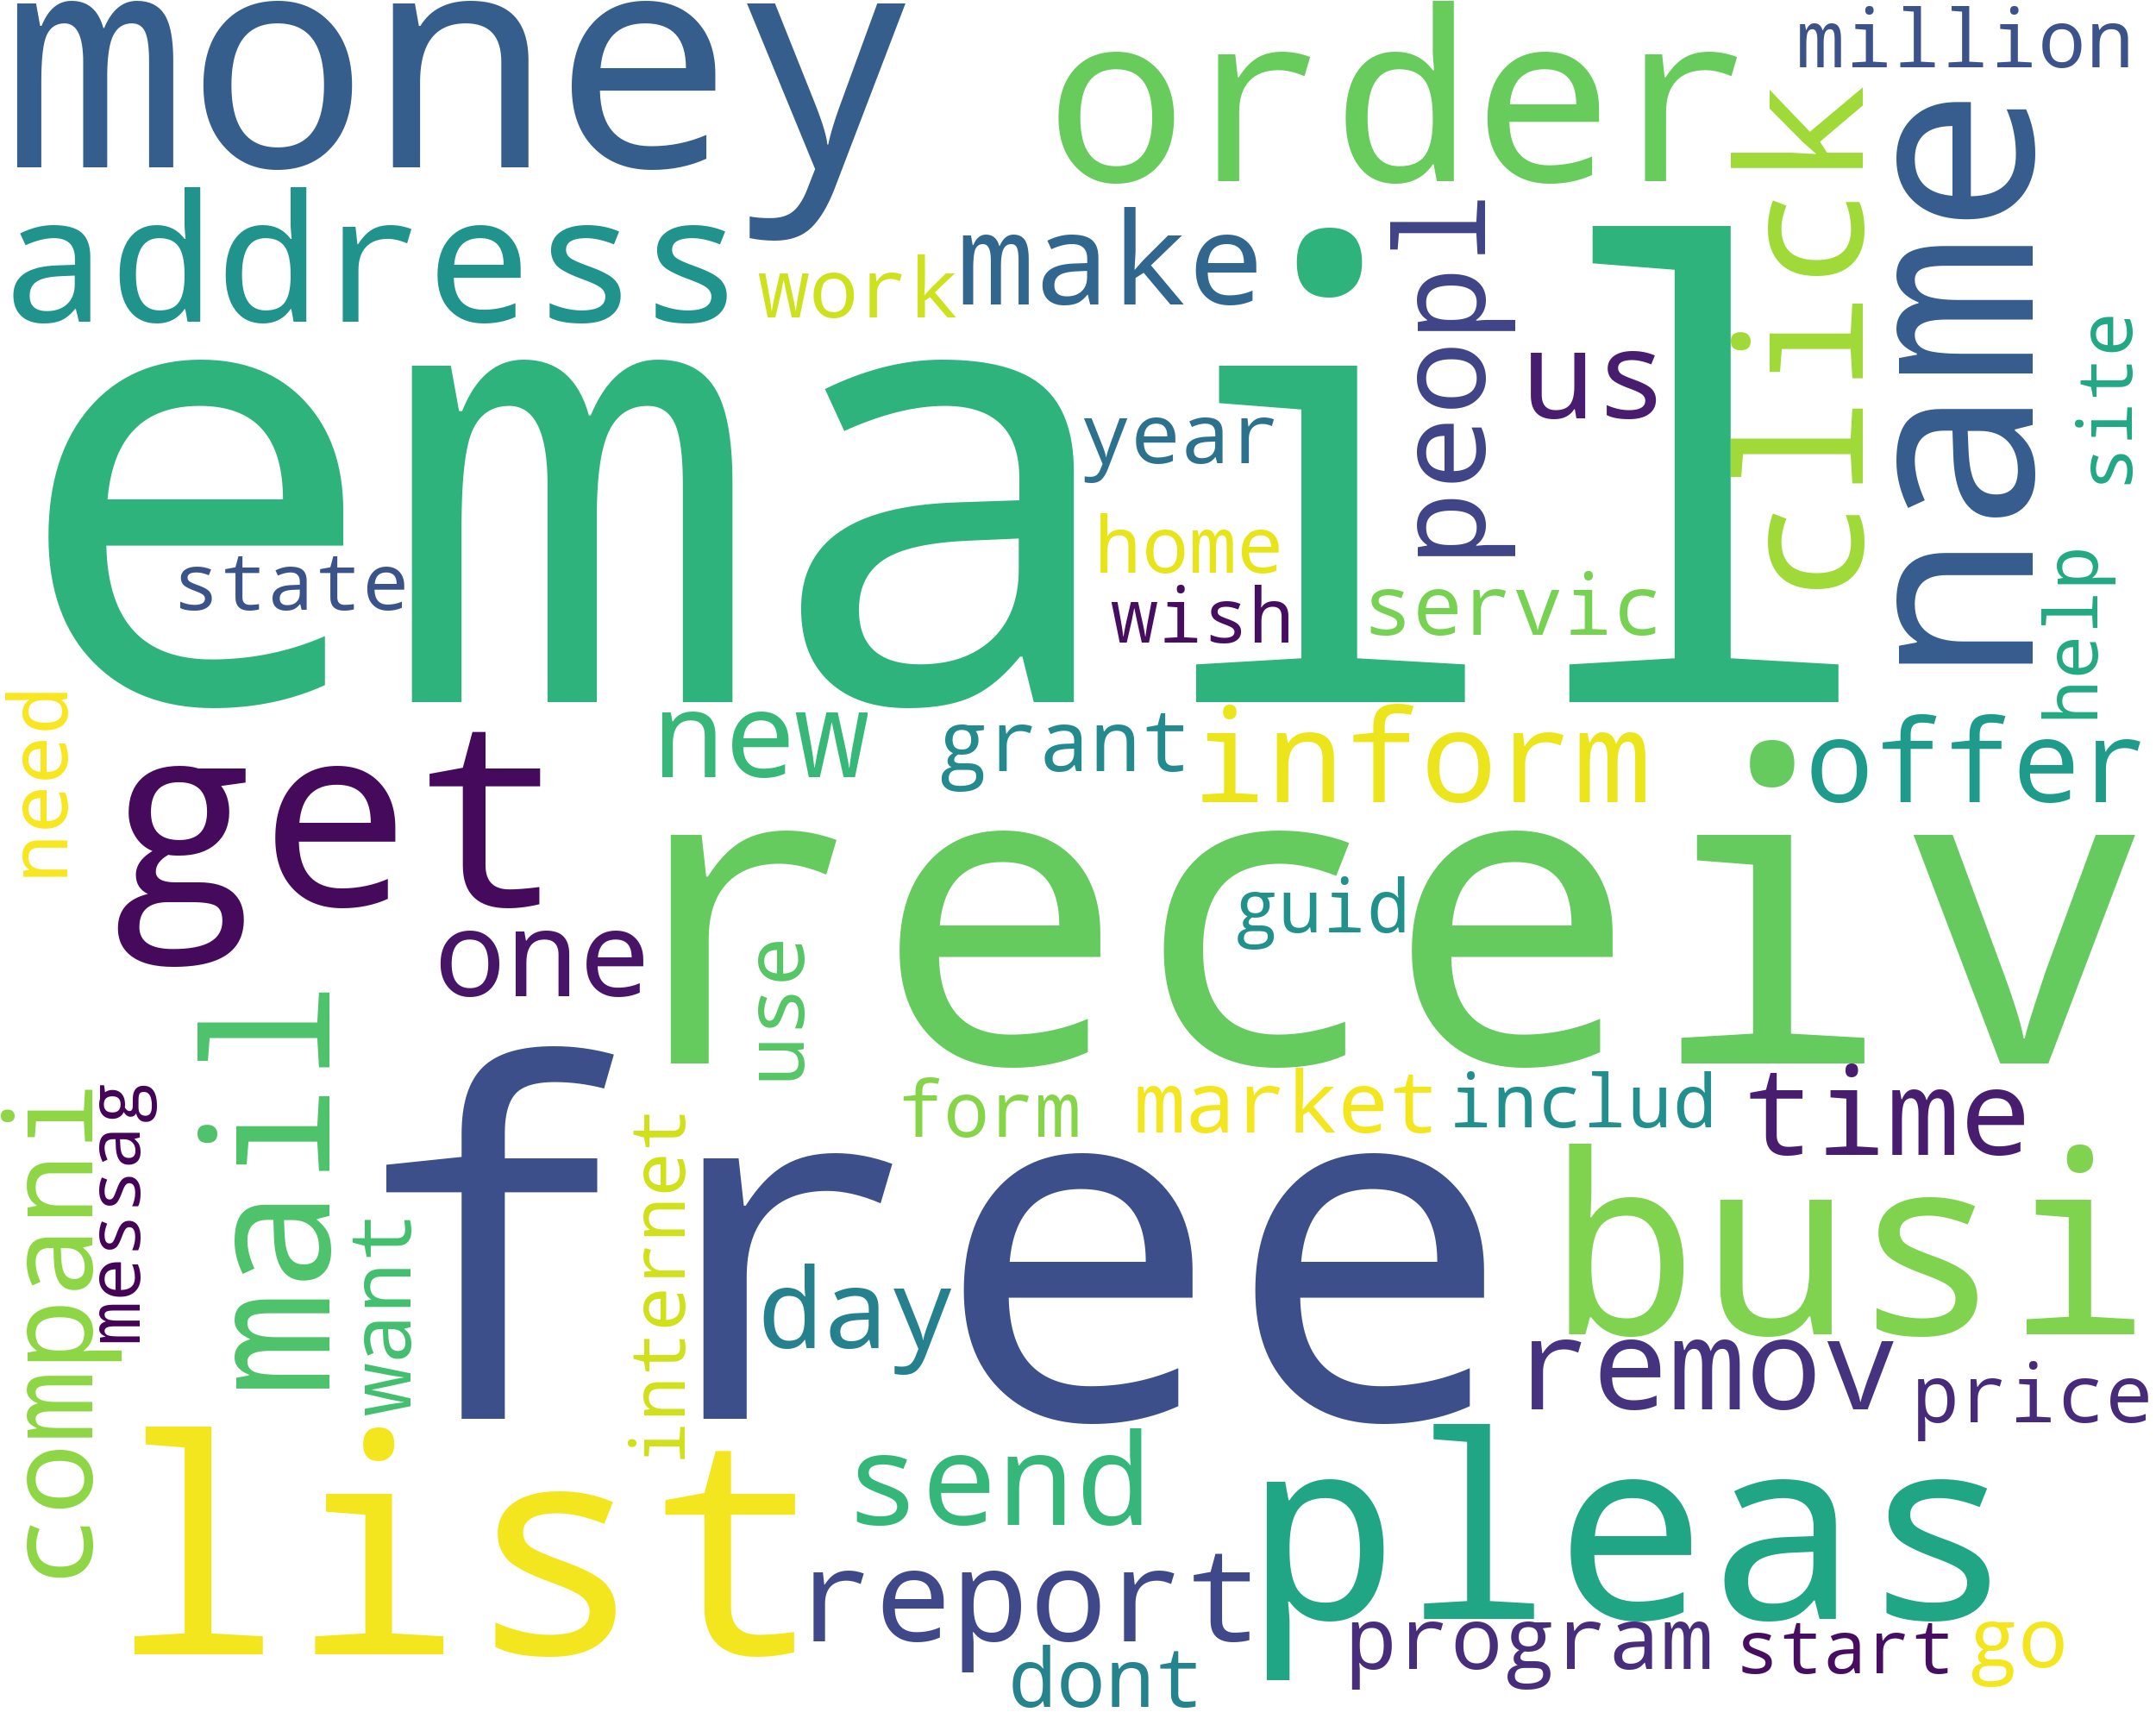
\includegraphics[width=\textwidth]{figures/spam_wc}
                \captionof{figure}{Spam}
                \label{spam_wc}
            \end{minipage}
            \begin{minipage}{0.4\columnwidth}
                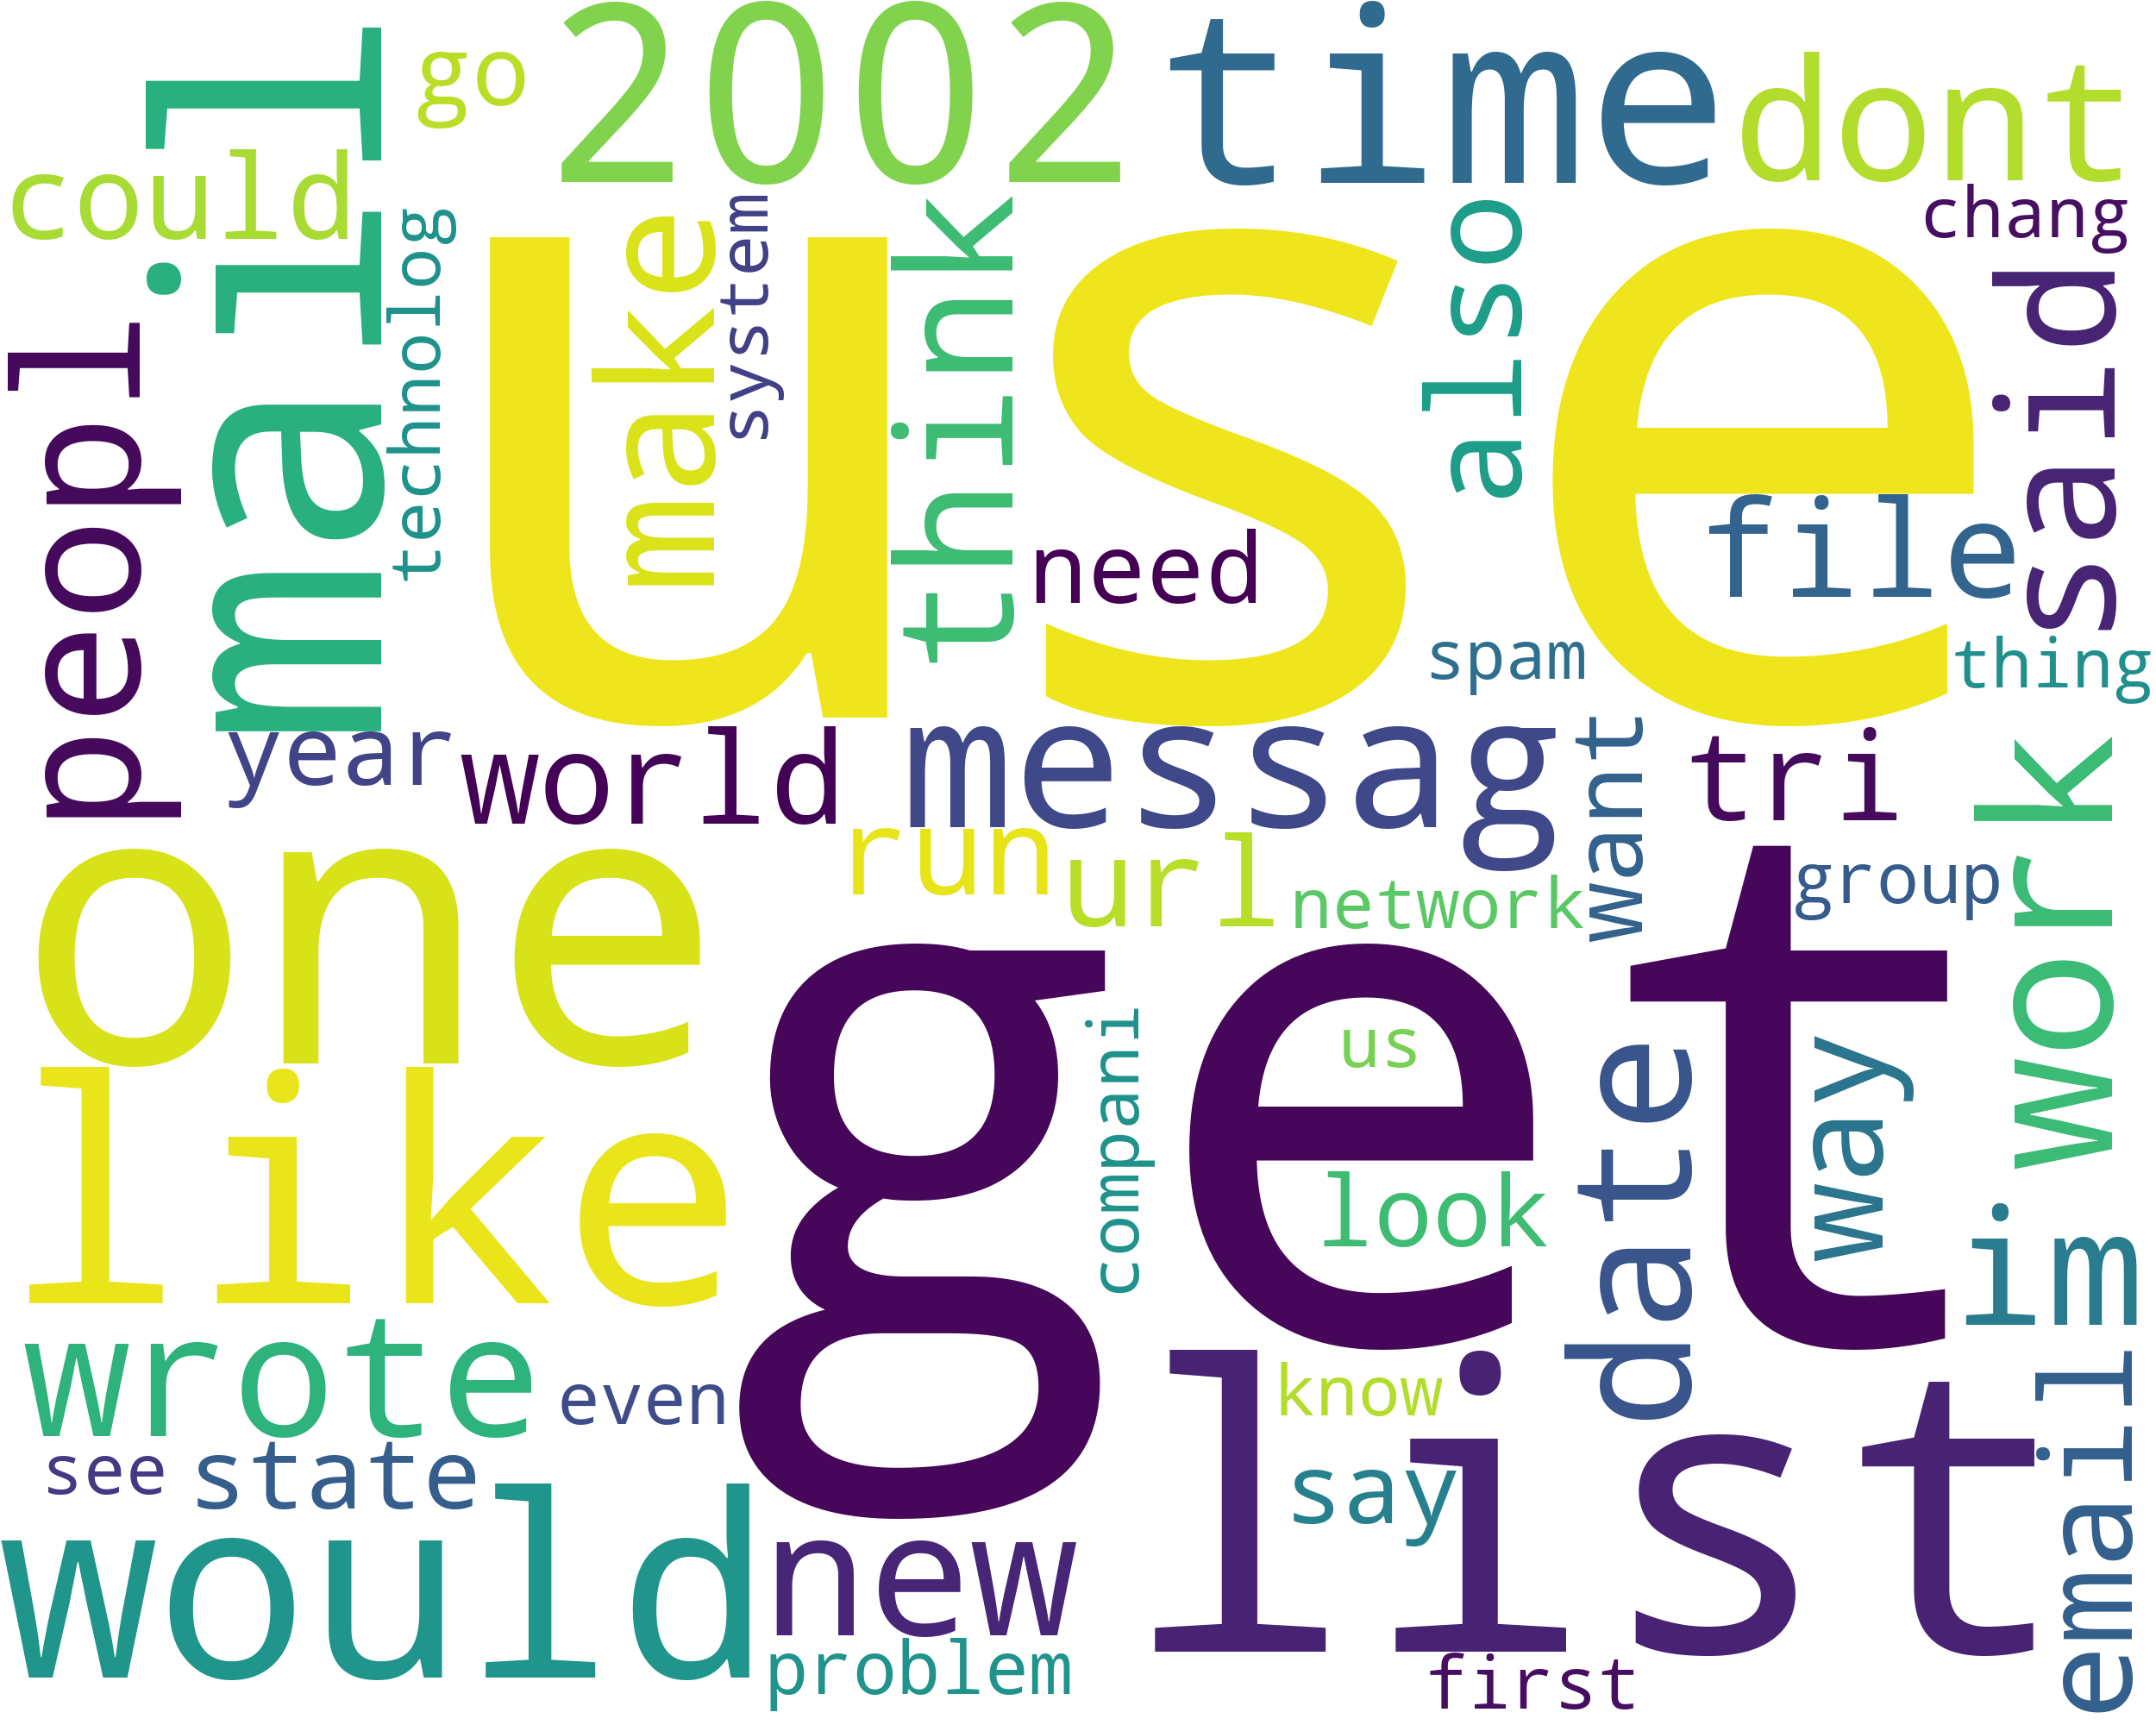
\includegraphics[width=\textwidth]{figures/ham_wc}
                \captionof{figure}{Ham}
                \label{ham_wc}
             \end{minipage}
            This is more text
        %\section{Classifier Selection}

        %\section{Classifier Tuning}

        %\section{Results}

        %\section{Evaluation}

        %\section{Conclusion}

        %\section{References}
        % \printbibliography
    \end{multicols}
\end{document}